\documentclass{report}
\usepackage[utf8]{inputenc}
\usepackage[Bjornstrup]{fncychap}
\usepackage{graphicx}
\usepackage{xcolor} % to access the named colour LightGray
\definecolor{LightGray}{gray}{0.9}
\usepackage{listings}
\usepackage[spanish]{babel}
\usepackage{apacite}
\usepackage{array}
\usepackage{minted}
\usepackage{caption}
\usepackage{hyperref}
\usepackage{listings}
\usepackage{xcolor}

\definecolor{codegreen}{rgb}{0,0.6,0}
\definecolor{codegray}{rgb}{0.5,0.5,0.5}
\definecolor{codepurple}{rgb}{0.58,0,0.82}
\definecolor{backcolour}{rgb}{0.95,0.95,0.92}

\lstdefinestyle{mystyle}{
    backgroundcolor=\color{backcolour},
    commentstyle=\color{codegreen},
    keywordstyle=\color{magenta},
    numberstyle=\tiny\color{codegray},
    stringstyle=\color{codepurple},
    basicstyle=\ttfamily\footnotesize,
    breakatwhitespace=false,
    breaklines=true,
    captionpos=b,
    keepspaces=true,
    numbers=left,
    numbersep=5pt,
    showspaces=false,
    showstringspaces=false,
    showtabs=false,
    tabsize=2
}
\lstset{style=mystyle}
\bibliographystyle{apacite}
\selectlanguage{spanish}
{
  \setlength{\columnsep}{4mm}
  \setlength{\parindent}{0.5in}
  \setlength{\parskip}{1em}
  \renewcommand{\baselinestretch}{1.5}
  \setlength{\headheight}{33pt}

  \thispagestyle{empty}
			\begin{figure}[ht]
				\minipage{0.87\textwidth}
					 
\includegraphics[width=2cm]{fi.jpg}
					 \label{escudoFI}
				\endminipage
				\minipage{0.32\textwidth}
					 
\includegraphics[height = 2.25cm ,width=2cm]{unam.png}
					 \label{EscuoUNAM}
				 \endminipage
					 %%\vspace{-1cm}
			 \end{figure}
			 
			 \vspace{0.1cm}
			 
			 \begin{center}
				 {\scshape\LARGE \textbf{Universidad Nacional Autónoma de México} \par}
				 {\scshape\Large Facultad de Ingeniería\par}
				 
				  {\Large ESTRUCTURAS DE DATOS Y ALGORITMOS II}
	 
				 % Restauramos el interlineado:
				 \begin{center}
				 
				 {\LARGE \textit{Grupo: 07 - Semestre: 2024-1}}
	 
				 

				 {\LARGE\bfseries PROYECTO 2 – ALGORITMOS DE BÚSQUEDA\par}
	 
			 {\scshape\Large Fecha de entrega: 08/10/2023\par}	
	 
						 \LARGE	{ \textbf{Profesor:}}\\%% \textbf son negritas
			 \large		{ Edgar Tista Garcia}
			 
			 \vspace{-0.5cm}	
			 
			 \LARGE	{ \textbf{Alumno(s):}}\\%% \textbf son negritas
	 
			 \normalsize	 {Hernandez Gallardo Daniel Alonso}
			 
			 \vspace{-0.5cm}
			 
			 \normalsize		{Perez Osorio Luis Eduardo}
			 
			 \vspace{-0.5cm}
			 
			 \normalsize		{Valle Chavez Anton Yael}
			 
			 
	 %% \it es letra itálica
					 \vspace{1.25cm}
					 \vspace{0.9cm}
					 
				 \end{center}
		 
			 \end{center} 
}

\addto\captionsspanish{\renewcommand{\abstractname}{Abstract}}
\begin{document}





  

 


  \begin{abstract}
This project is based on prior research that focuses on the main collections in Java and their class hierarchies. In this research, implementations of lists, hash tables, and sets in Java are explored, along with their key differences.

The class hierarchy in Java starts with the java.util.Collection interface, which has subinterfaces such as List, Set, and Map. Each of these subinterfaces represents different types of collections with unique characteristics. For instance, List allows duplicates and maintains a specific order, Set disallows duplicates, and Map represents a collection of key-value pairs.

Within these categories, specific implementations were investigated. Regarding lists, ArrayList, LinkedList, and Vector were examined, each with its advantages and specific use cases. In the context of hash tables, HashMap, LinkedHashMap, and TreeMap were considered, offering varying levels of performance and ordering. Additionally, in the realm of sets, HashSet, LinkedHashSet, and TreeSet were explored, each with its own duplication and ordering characteristics.

This research lays the foundation for understanding data structures and collections in Java, which is essential for the development of search and chaining applications. The programs implement key comparison search algorithms such as linear search and binary search, in the context of comparable objects like Students and Subjects. Furthermore, collision resolution is explored through chaining in a simulated hash table, and an interactive interface is created to allow users to add elements to the table and view its contents.
  \end{abstract}
    

 
  \section*{Resumen}
 Este proyecto se basa en una investigación previa que se centra en las principales colecciones en Java y sus jerarquías de clases. En esta investigación, se exploran las implementaciones de listas, tablas hash y conjuntos (Set) en Java, así como las diferencias clave entre ellas.

La jerarquía de clases en Java comienza con la interfaz java.util.Collection, que tiene subinterfaces como List, Set y Map. Cada una de estas subinterfaces representa diferentes tipos de colecciones con características únicas. Por ejemplo, List permite duplicados y mantiene un orden específico, Set no permite duplicados y Map representa una colección de pares clave-valor.

Dentro de estas categorías, se investigaron las implementaciones específicas. En el caso de listas, se examinaron ArrayList, LinkedList y Vector, cada una con sus ventajas y casos de uso particulares. En cuanto a las tablas hash, se consideraron HashMap, LinkedHashMap y TreeMap, que ofrecen diferentes niveles de rendimiento y ordenación. Además, en el contexto de conjuntos, se exploraron HashSet, LinkedHashSet y TreeSet, cada uno con sus propias características de duplicación y orden.

Esta investigación sienta las bases para comprender las estructuras de datos y las colecciones en Java, lo que es esencial para el desarrollo de las aplicaciones de búsqueda y encadenamiento. Los programas implementan algoritmos de búsqueda por comparación de llaves, como búsqueda lineal y búsqueda binaria, en el contexto de objetos comparables, como Alumnos y Asignaturas. Además, se explora la solución de colisiones mediante el encadenamiento en una tabla hash simulada y se crea una interfaz interactiva para permitir a los usuarios agregar elementos a la tabla y ver su contenido.



\tableofcontents

  

\chapter{Introducción} 
    \section*{Objetivo}
    Que el alumno desarrolle aplicaciones para la búsqueda por comparación de llaves y la
    transformación de llaves junto con la solución de colisiones
    \section*{investigación}
      \subsection*{Framework}
      Un framework es una agrupación de clases e interfaces que proporcionan una arquitectura lista para desarrollar software. Por ende, si se quiere implementar una nueva característica o clase, no es necesario definir un nuevo framework si ya existe uno. No obstante, una buena práctica en el paradigma orientado a objetos es incluir un framework con una colección de clases tal que todas las clases realicen el mismo tipo de operaciones.
      \subsection*{Colecciones en Java}
      Cualquier grupo de objetos individuales que se representa como una sola unidad se le conoce como una colección de objetos. En el lenguaje de programación Java, en Java Development Kit 1.2 se definió un modelo denominado Collection Framework que contiene todas las clases de colección con sus respectivas interfaces. De ahí que la interfaz de colección java.util.Collection y la interfaz de mapa java.util.Map son las dos interfaces principales de las clases de colección en Java.
      \subsection*{Collection Framework en Java}
      Antes de que existiera el Collection Framework, es decir, antes de JDK 1.2, los métodos estándar para agrupar objetos en Java, o colecciones, eran Arrays, Vectors o Hashtables. Todas estas colecciones no tenían una interfaz en común. Por consiguiente, aunque el objetivo principal de todas las colecciones es el mismo, la implementación de todas estas colecciones se definió de forma independiente y en consecuencia no había ninguna relación entre ellas. Además, era muy difícil para los programadores recordar los diferentes métodos, sintaxis y constructores existentes para cada clase de colección.
      \subsection*{Ventajas del Collection Framework en Java}
      Como ya se mencionó anteriormente, la falta de un framework dio lugar a las desventajas descritas en la sección anterior. Sin embargo, luego de que se declaró el framework se comenzaron a presentar ventajas.
      \begin{itemize}
          \item \textbf{API consistente:} la API tiene un conjunto básico de interfaces como Collection, Set, List o Map, donde todas las clases, ArrayList, LinkedList, Vector, que implementan estas interfaces tienen métodos en común.
          \item \textbf{Reduce la complejidad al programar:} un programador ya no tiene que preocuparse por el diseño de la Colección, lo cual le permite priorizar el resto de su programa. Por lo anterior, uno de los principales aspectos del paradigma orientado a objetos, el cual es abstracción se logró implementar satisfactoriamente.
          \item \textbf{Aumenta la eficiencia y la calidad del programa:} la eficiencia se ve incrementada gracias a la proporción de implementaciones de alto rendimiento para las estructuras de datos junto con algunos algoritmos útiles, ya que, en este caso, el programador no necesita preocuparse por elegir la mejor implementación de una estructura de datos particular. Simplemente puede utilizar la implementación predefinida y así aumentar el rendimiento de su algoritmo/programa.
      \end{itemize}
      \newpage
      \subsection*{Jerarquía del Collection Framework en Java}El paquete java.util contiene todas las clases e interfaces que requiere el Collection Framework. Asimismo, el Collection Framework contiene una interfaz conocida como Iterable, la cual proporciona un iterador para recorrer todas las colecciones. Todas las colecciones que amplían la interfaz, aumentan al mismo tiempo el rango del iterador y los métodos de esta. La siguiente imagen ilustra la jerarquía del Collection Framework.
    \begin{figure}[h]
    \centering
    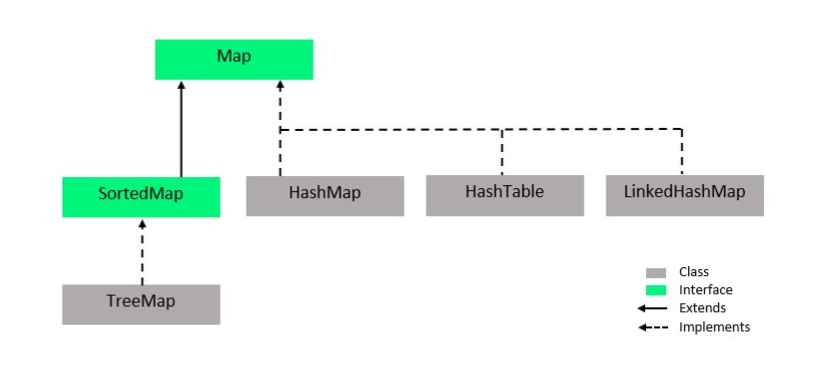
\includegraphics[width=1\linewidth]{Collection-Framework-2.png}
    \caption{GeeksforGeeks. (2023). Jerarquía del Collection Framework en Java[PNG].GeeksforGeeks
\href{https://media.geeksforgeeks.org/wp-content/uploads/20230124151239/Collections-in-Java-768.png}{https://media.geeksforgeeks.org/wp-content/cdn-uploads/20200811210521/Collection-Framework-1.png}.}
\end{figure}

\begin{figure}[h]
    \centering
    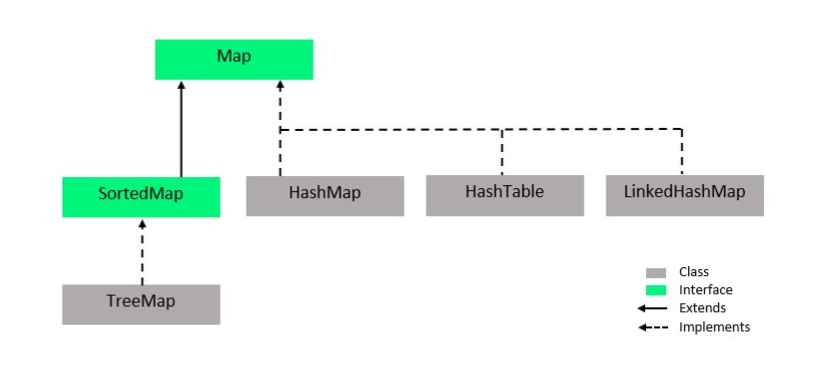
\includegraphics[width=0.75\linewidth]{Collection-Framework-2.png}
    \caption{GeeksforGeeks. (2023). Jerarquía del Collection Framework en Java [PNG]. GeeksforGeeks https://media.geeksforgeeks.org/wp-content/cdn-uploads/20200811210611/Collection-Framework-2.png. }
\end{figure}
\newpage
Antes de profundizar en los diferentes componentes del modelo, es importante recordar los conceptos de clase e interfaz.
\begin{itemize}
    \item \textbf{Clase:}una clase es un modelo o prototipo definido por el usuario a partir del cual se van a crear objetos. En esta, se representa un conjunto de atributos y métodos que serán comunes para todos los objetos de la clase.

    \item \textbf{Interfaz:} al igual que una clase, una interfaz puede tener métodos y atributos, pero los métodos declarados en una interfaz son abstractos por defecto. Entonces, las interfaces especifican qué debe hacer una clase más no el cómo, es decir, son la plantilla de la clase.
\end{itemize}
    \subsection*{Clase contra Interfaz}
    
    
\begin{table}[h]
\centering
\begin{tabular}{|p{7cm}|p{7cm}|} 
\hline  
\textbf{Clase} & \textbf{Interfaz}\\ 
\hline  
Una clase es un prototipo definido por el usuario para construir objetos en Java.& Una interfaz es un modelo definido por el usuario que describe la estructura de cada clase que la implementa.\\ 
\hline  
Una interfaz es un modelo definido por el usuario que describe la estructura de cada clase que la implementa.& No se puede utilizar para instanciar objetos.\\ 
\hline  
Una clase puede tener modificadores de acceso públicos y predeterminados.& Una Interfaz puede tener modificadores de acceso públicos y predeterminados.\\ 
\hline  
Las clases pueden ser concretas o abstractas.& Todas las interfaces son abstractas.\\ 
\hline  
Una clase consta de constructores, métodos y atributos. Los métodos están definidos en una clase.& Una interfaz consta de atributos y métodos. Los métodos no están definidos en una interfaz, sólo contiene sus prototipos.\\ 
\hline 
\end{tabular}
\caption{Comparación entre Clase e Interfaz en Java}
\label{tab:my_label}
\end{table}
\subsection*{Métodos de la interfaz Collection}
Esta interfaz contiene varios métodos que pueden ser utilizados por todas las colecciones que implementan esta interfaz. Los cuales son:
\begin{itemize}
    \item \textbf{add(Object)} se utiliza para agregar un objeto a la colección.
    \item \textbf{addAll(Collection c)} agrega todos los elementos de la colección que se recibe como parámetro a la colección.
    \item \textbf{clear()} elimina todos los elementos de la colección.
    \item \textbf{contains(Object o)} devuelve verdadero si la colección contiene el objeto especificado.
    \item \textbf{containsAll(Collection c) }devuelve verdadero si la colección contiene todos los elementos de la colección que recibe como parámetro.
    \item \textbf{equals(Object o)} compara el objeto especificado con la colección para determinar la igualdad.
    \item \textbf{hashCode()} se utiliza para devolver el valor del código hash para esta colección, es decir, el identificador de 32 bits que se almacena en un Hash en la instancia de la clase.
    \item \textbf{isEmpty()} devuelve verdadero si la colección no contiene elementos.
    \item \textbf{iterator()} devuelve un iterador sobre los elementos de esta colección.
    \item \textbf{max()} se utiliza para devolver el valor máximo presente en la colección.
    \item \textbf{parallelStream()} devuelve un Stream paralelo con esta colección como fuente, dicho de otra manera, este genera un Stream donde cada elemento no depende de otro para ser procesado.
    \item \textbf{remove(Object o)} se utiliza para eliminar el objeto dado de la colección. Sin embargo, si hay valores duplicados, este método elimina la primera aparición del objeto.
    \item \textbf{removeAll(Collection c)} se utiliza para eliminar de la colección todos los objetos contenidos en la colección que recibe como parámetro.
    \item \textbf{removeIf(Predicate filter)} se utiliza para eliminar todos los elementos de esta colección que satisfacen el predicado dado.
    \item \textbf{retainAll(Collection c)} se utiliza para conservar sólo los elementos de la colección que están contenidos en la colección especificada.
    \item \textbf{size()} se utiliza para conocer la cantidad de elementos de la colección.
    \item \textbf{spliterator()} se utiliza para crear un Spliterator sobre los elementos de esta colección, el cual nos permite recorrer y dividir una secuencia de elementos.
    \item \textbf{stream()} devuelve un Stream secuencial con la  colección como fuente, el cual permite operar con la colección y hacer que el procesamiento masivo de datos sea rápido y fácil de leer.
    \item \textbf{toArray()} devuelve un array que contiene todos los elementos de la colección.
\end{itemize}
    \subsection*{Interfaces y clases del Collection Framework}
     
    \subsubsection*{Interfaz Iterable}
Esta interfaz es la raíz de todo el Collection Framework. Como se observa en la imagen, la interfaz de Collection amplía la interfaz Iterable. Por lo tanto, todas las interfaces y clases implementan esta interfaz. La función principal de esta interfaz es proporcionar un iterador para las colecciones. De ahí que, esta interfaz contiene sólo un método abstracto que es el iterador.
\subsubsection{Interfaz Collection}
Como ya se mencionó, esta interfaz amplía la interfaz Iterable y a su vez amplia la implementación de todas las clases en el Collection Framework. Esta interfaz contiene todos los métodos básicos que tiene cada colección, como agregar datos a la colección, eliminar datos, borrar datos. Todos estos métodos se implementan en esta interfaz porque estos son usados por todas las clases independientemente de su lógica. Además, tener estos métodos en esta interfaz garantiza que los nombres de los métodos sean universales para todas las colecciones. Por consiguiente, esta interfaz construye una base sobre la cual se implementan las clases del resto de interfaces.
\subsubsection{Interfaz List}
Esta es una interfaz secundaria de la interfaz de Collection. Se enfoca en las clases que son una colección secuencial en la que el usuario de la interfaz tiene control sobre cualquier elemento que es insertado a la lista. Además, el usuario puede acceder a sus elementos por un índice entero o buscar algún elemento en la lista. Por otra parte, a diferencia de la interfaz Set, la interfaz List si permite que haya elementos repetidos junto con varios elementos nulos. De ahí que esta interfaz está implementada por clases como ArrayList, Vector, Stack y LinkedList. En consecuencia, podemos crear una instancia de un objeto de List con cualquiera de las clases mencionadas.
\paragraph{Clase ArrayList}
Esta clase implementa una lista como un arreglo al que se le puede cambiar el tamaño, junto con todas las operaciones opcionales de la lista e igual permite todos los elementos, incluido null. Asimismo, provee métodos que manipulan el tamaño del arreglo interno usado para almacenar la lista. Por lo que, esta clase es similar a la clase Vector, solo que no está sincronizada, es decir, que múltiples subprocesos pueden operar en un ArrayList al mismo tiempo para hacer un ArrayList seguro para subprocesos. Sin embargo, se puede sincronizar externamente usando el método Collections.synchronizedList().
\paragraph{Clase Vector}
Esta clase implementa una variedad creciente de objetos. Al igual que una matriz, contiene elementos a los que se puede acceder mediante un índice entero. Sin embargo, el tamaño de un Vector puede aumentar o disminuir según se requiera para permitir las operaciones de adición y eliminación de elementos una vez que ya se creó un objeto de la clase. Al igual que la clase ArrayList, esta clase también permite todos los elementos, incluido null.  Además, como ya se mencionó anteriormente, la clase Vector si es sincronizada, lo cual implica que sólo un único subproceso puede operar en un método de Vector a la vez.
\paragraph{Clase Stack}
La clase Stack representa una pila de objetos donde el último en entrar, es el primero en salir (LIFO). Por ende, cuando se crea una pila por primera vez, no contiene elementos. Asimismo, amplía la clase Vector con cinco operaciones que permiten tratar un vector como una pila. 
\begin{itemize}
    \item \textbf{empty()} prueba si la pila está vacía.
    \item \textbf{peek() }mira el objeto en la parte superior de la pila sin sacarlo de la pila.
    \item \textbf{pop()} elimina el objeto en la parte superior de la pila y devuelve ese objeto como el valor de esta función.
    \item \textbf{push(E item)} agrega un elemento a la parte superior de la pila.
    \item \textbf{search(Object o)} devuelve la posición basada en 1 de donde se encuentra un objeto en la pila.
\end{itemize}
\paragraph{Clase LinkedList}
Esta clase es la implementación de una lista doblemente ligada de las interfaces List y Deque. Incluye todas las operaciones de lista opcionales y permite todos los elementos (incluido null). Además, todas las operaciones se realizan como se podría esperar en una lista doblemente ligada. Por otro lado, las operaciones que indexan la lista recorrerán la lista desde el principio o el final, de acuerdo con lo que esté más cerca del índice especificado. Hay que tener en cuenta que esta implementación no está sincronizada, es decir, si varios subprocesos acceden a una LinkedList al mismo tiempo y al menos uno de los subprocesos modifica la lista estructuralmente, debe sincronizarse externamente.

\subsubsection*{Aspectos a tomar en cuenta para elegir alguna de las clases de List}
Como se vio anteriormente, las clases ArrayList, LinkedList, Vector y Stack son todas implementaciones de la interfaz List, pero se utilizan en diferentes situaciones debido a sus características y rendimiento. Por ende, conviene tener en cuenta algunos aspectos para saber cuándo conviene usar cada una.
\begin{itemize}
    \item ArrayList:
    \begin{itemize}
     \item Se suele utilizar cuando se necesita una lista dinámica que se puede redimensionar y acceder rápidamente a sus elementos con un índice. En consecuencia, la clase ArrayList es la elección más común.
      \item En cuanto al rendimiento, esta clase ofrece un acceso rápido a elementos por índice, sin embargo, puede ser menos eficiente al insertar o eliminar elementos que se encuentran al medio de la lista debido a que se tienen que desplazar elementos.
    \end{itemize}


    \item LinkedList:
    \begin{itemize}
    \item Se recomienda utilizar cuando vas a insertar o eliminar de manera frecuente elementos al medio de la lista, ya que en este aspecto la clase LinkedList puede ser más eficiente que la clase ArrayList. También es útil cuando se requiere iterar sobre la lista en ambas direcciones, es decir del inicio al final o del final al inicio.
    \item Ahora bien, el rendimiento en cuanto a insertar y eliminar elementos en la clase LinkedList es más rápido que en la clase ArrayList, pero el acceso aleatorio es más lento.
        \end{itemize}
    \item Vector:
    \begin{itemize}
    \item Se utiliza con menos frecuencia en las aplicaciones modernas. Es similar a la clase ArrayList, pero esta clase si es sincronizada, lo que significa que es segura para el uso de hilos múltiples. Por ello, si necesitas una lista sincronizada, puedes considerar usar la clase Vector. De lo contrario, es preferible usar ArrayList.
    \item En lo que al rendimiento se refiere, a causa de la sincronización, la clase 
    Vector puede ser más lenta que la clase ArrayList en operaciones sin hilos múltiples.
      \end{itemize}
    \item Stack:
    \begin{itemize}
    \item Se recomienda usar si necesitas una estructura de datos tipo LIFO (Last In, First Out). Sin embargo, es preferible usar la interfaz Deque con la clase LinkedList o ArrayDeque en lugar de la clase Stack, ya que el uso de esta clase no se aconseja desde Java 1.5.
    
    \item El rendimiento suele ser aceptable para operaciones de apilar y desapilar, no obstante, se debe tener en cuenta que la interfaz Deque ofrece una mayor flexibilidad y opciones.
      \end{itemize}
\end{itemize}
\subsubsection{Interfaz Queue}
La interfaz Queue mantiene la lógica FIFO donde el primero en entrar, es el primero en salir, lo cual es similar a una cola de espera en el mundo real. Por ello, esta interfaz está dedicada a almacenar elementos donde el orden de los elementos sí importa. Por ejemplo, cuando queremos reservar un boleto, los boletos se venden por orden de llegada. Por lo tanto, la persona cuya solicitud llega primero a la cola obtiene el billete antes que los demás. En este sentido, hay clases como PriorityQueue, ArrayDeque y LinkedList para implementar la interfaz Queue, por lo que, se puede crear una instancia con cualquiera de estas clases.
\paragraph{Clase PriorityQueue}
Esta clase permite usar la lógica de una cola de prioridad ilimitada, la cual se basa en un Heap de prioridad. Además, los elementos de la cola de prioridad se ordenan según su orden natural, o de acuerdo con un parámetro Comparator proporcionado en el momento de la construcción de la cola, conforme al constructor que se utilice. Lamentablemente, la PriorityQueue no permite elementos null. Asimismo, como se basa en el orden natural tampoco permite la inserción de objetos no comparables, ya que hacerlo puede resultar en ClassCastException.
\paragraph{Interfaz Deque}
Esta es una variación muy ligera de la interfaz Queue. Por ende, la interfaz Deque, también conocida como cola doble, es una interfaz con la que podemos agregar y eliminar elementos de ambos extremos de la cola. Como ya se mencionó, la interfaz Deque amplía la interfaz Queue. Por otro lado, las clases que implementan esta interfaz son ArrayDeque y LinkedList, por lo cual, podemos crear una instancia de alguna de estas clases.
\paragraph{Clase ArrayDeque}
Esta clase implementa un array redimensionable con la interfaz Deque que a su vez amplía la interfaz Queue. Un ArrayDeque no tiene restricciones de capacidad, porque crece según sea necesario para soportar el uso. Sin embargo, no son seguros para subprocesos, ya que en ausencia de sincronización externa, no admiten el acceso simultáneo de varios subprocesos. Además, los elementos nulos están prohibidos en esta clase. A pesar de lo anterior, es probable que esta clase sea más rápida que la clase Stack cuando se usa como pila y más rápida que la clase LinkedList cuando se usa como cola.
\paragraph{Clase LinkedList}
Esta clase es la implementación de una lista doblemente ligada de las interfaces List y Deque, la cual a su vez amplía la interfaz Queue. Incluye todas las operaciones de lista opcionales y permite todos los elementos (incluido null). Además, si se usa como una cola todas las operaciones se realizan como se podría esperar. Por otra parte, las operaciones que indexan la cola permiten recorrerla de inicio a fin o viceversa, según se requiera. Nuevamente, se debe tener en cuenta que esta implementación no está sincronizada, por lo cual, si varios subprocesos acceden a una LinkedList al mismo tiempo y al menos uno de los subprocesos modifica la lista estructuralmente, debe sincronizarse externamente.

\subsubsection{Aspectos a tomar en cuenta para elegir alguna de las clases de Queue}
De acuerdo con lo ya mencionado, elegir alguna de las clases PriorityQueue, ArrayDeque o LinkedList para implementar la interfaz Queue depende de nuestras necesidades y de las operaciones que planeamos realizar con la estructura de datos cola. Por consiguiente, conviene tener en cuenta algunos aspectos para determinar la clase que más nos convendrá usar para determinada aplicación.
\begin{itemize}
    \item PriorityQueue:
    \begin{itemize}
    \item Se recomienda usar cuando necesitas una cola de prioridad, es decir, cuando quieres que los elementos se almacenen y recuperen según un orden específico definido por su prioridad. Por lo anterior, los elementos se recuperan de la cola en orden ascendente o descendente de acuerdo con la prioridad que se haya definido.
    \item En lo que al rendimiento se refiere, la PriorityQueue es eficiente para insertar y eliminar elementos según su prioridad, pero no es eficiente si necesitas acceder a elementos en posiciones arbitrarias o si la prioridad de los elementos cambia con frecuencia.
    \end{itemize}
    \item ArrayDeque:
    \begin{itemize}
    \item Cuándo quieres una cola doble para insertar y eliminar elementos de manera eficiente tanto al principio como al final, entonces la clase ArrayDeque es una excelente opción. Por otra parte, un objeto de esta clase se puede usar como una cola FIFO o una pila LIFO según tus necesidades.
    \item El rendimiento de la clase ArrayDeque es muy eficiente para operaciones de inserción y eliminación en ambos extremos de la cola, pero no brinda un orden basado en una prioridad como la clase PriorityQueue.
    \end{itemize}
    \item LinkedList:
    \begin{itemize}
    \item Un objeto de la clase LinkedList puede usarse para implementar una cola FIFO o una pila LIFO. Sin embargo, generalmente es menos eficiente que la clase ArrayDeque para estas operaciones. A pesar de lo anterior, puedes considerar usar la clase LinkedList si necesitas una cola y también si deseas acceder a elementos en posiciones arbitrarias con frecuencia.
    \item Respecto al rendimiento, la clase LinkedList es menos eficiente que la clase ArrayDeque para operaciones de inserción y eliminación en los extremos de la cola, pero es mejor si necesitas acceder a alimentos aleatorios.
    \end{itemize}
\end{itemize}
\subsubsection{Interfaz Set}
Un set es una colección desordenada de objetos en la que no se pueden almacenar elementos duplicados, es decir, un set no posee dos elementos e1 y e2 tal que se pueda usar el método e1.equals(e2). Esta interfaz se utiliza cuando deseamos evitar la duplicación de los objetos y deseamos almacenar sólo objetos únicos, con máximo un elemento nulo, puesto que, esta colección modela la abstracción matemática de un conjunto. Por ello, esta interfaz se puede implementar mediante  la creación de una instancia de alguna clase como HashSet, TreeSet y LinkedHashSet.
\paragraph{Clase HashSet}
Esta clase implementa la interfaz Set, y a su vez está respaldada por una tabla hash, la cual en realidad es una instancia de la clase HashMap. Sin embargo, esta clase no ofrece garantía en cuanto al orden de iteración del conjunto; en particular, no garantiza que el orden se mantendrá constante en el tiempo. Asimismo, esta clase si permite el elemento null. Por otra parte, tiene un rendimiento de tiempo constante para las operaciones de inserción y eliminación promedio. Finalmente, hay que tener en cuenta que esta implementación no está sincronizada, dicho de otra forma, si varios subprocesos acceden a un HashSet al mismo tiempo y al menos uno de los subprocesos lo modifica, se debe sincronizar externamente.
Por lo general, esto se logra mediante la sincronización de algún objeto que encapsule naturalmente el HashSet. Si no existe tal objeto, el HashSet debe ajustarse utilizando el método Collections.synchronizedSet. Es mejor hacerlo en el momento de la creación, para evitar el acceso accidental y no sincronizado al HashSet.
\paragraph{Clase LinkedHashSet}
Esta clase es la implementación de una tabla hash y una lista ligada de la interfaz Set, por lo cual, tiene un orden de iteración predecible. A diferencia de la clase HashSet, la clase LinkedHashSet mantiene una lista doblemente ligada que recorre todas sus entradas. Por lo cual, esta lista doblemente ligada define el orden de iteración, el cual es el orden en el que se insertaron los elementos en el Set. No hay que perder de vista que el orden de inserción no se ve afectado si un elemento se vuelve a insertar en el LinkedHashSet. En consecuencia, esta implementación evita los pedidos no especificados y generalmente caóticos que se generan con la clase HashSet, sin incurrir en el mayor costo asociado con la clase TreeSet.
Por lo anterior, se puede utilizar la clase LinkedHashSet para generar una copia de un Set que tenga el mismo orden que el original, independientemente de la implementación del conjunto original.
\subsubsection{Interfaz SortedSet}
Esta interfaz es muy similar a la interfaz Set. La única diferencia es que esta interfaz tiene métodos adicionales que mantienen el orden de los elementos. Por consiguiente, la interfaz SortedSet amplía la interfaz Set y se utiliza para manejar los datos que deben ordenarse. La clase que implementa esta interfaz es TreeSet, por lo que se puede crear una instancia con esta clase para usar la interfaz SortedSet.
\subsubsection{Interfaz NavigableSet}
La interfaz NavigableSet se extiende desde la interfaz SortedSet. Además de los métodos de la interfaz SortedSet, la interfaz NavigableSet tiene métodos de navegación que brindan coincidencias más cercanas, como floor, ceiling, lower y higher. Un NavigableSet se puede recorrer en orden ascendente y descendente. Aunque permite el uso elementos nulos, no se recomienda, ya que estos elementos pueden generar resultados ambiguos.
\paragraph{Clase TreeSet}
Esta clase implementa la interfaz Set, SortedSet y NavigableSet utilizando una estructura de árbol, normalmente un Red-Black Tree, pues se usa para administrar el orden. Por defecto, se tiene un orden ascendente, pero se puede cambiar usando un Comparator. Además, su complejidad temporal asintótica es de O(log n) para sus operaciones de inserción, eliminación y búsqueda. Por otra parte, al igual que la clase HashSet esta clase tampoco es sincronizada, por lo que, si se quiere sincronizar se debe hacer de la misma forma que se hace con un objeto de la clase HashSet. Además, dada la naturaleza de este Set, se tienen algunos métodos exclusivos a la hora de implementarlo.
\begin{itemize}
    \item \textbf{ceiling(E element)} devuelve el elemento más pequeño en el conjunto que es mayor o igual al elemento especificado.
    \item \textbf{floor(E element)} devuelve el elemento más grande en el conjunto que es menor o igual al elemento especificado.
    \item \textbf{higher(E element)} devuelve el elemento más pequeño en el conjunto que es estrictamente mayor que el elemento especificado.
    \item \textbf{lower(E element)} devuelve el elemento más grande en el conjunto que es estrictamente menor que el elemento especificado.
    \item \textbf{pollFirst()} recupera y elimina el primer elemento más pequeño en el conjunto.
    \item \textbf{pollLast()} recupera y elimina el último elemento más grande en el conjunto.
    \item \textbf{descendingSet()} devuelve una vista inversa del conjunto, donde los elementos se almacenan en orden inverso.
\end{itemize}

\subsubsection{Aspectos a tomar en cuenta para elegir alguna de las clases de Set}
Para las clases mencionadas anteriormente, se debe definir cuál queremos usar según el problema que se nos presente y que encaje con las características especiales de cada Set. Por ejemplo, en el siguiente problema (B. Sereja and Suffixes Codeforces Problem 368B):
Se nos presenta una situación en la que se nos da un conjunto de números que tiene cualquier orden y contiene números repetidos, y se no da otro conjunto de números que representan índices del anterior conjunto de números brindados, queremos saber la cantidad de números diferentes que se encuentren después de cada índice que se nos ha brindado, además el problema debe ser solucionado en máximo un segundo para entradas de 105.
La situación es clara, necesitamos un Set, pues la respuesta será su tamaño después de recorrer la colección de números desde el índice brindado, pero además de esto necesitamos que el Set sea rápido al momento de realizar sus operaciones para cumplir con el límite de un segundo, y la clase de la interfaz Set que cumple con estas características es el HashSet, dado que este tiene las operaciones más rápidas y a su vez cumple con la función, como el resto de clases en la interfaz, de no admitir números repetidos. Por lo anterior, el código en el lenguaje de programación Java queda de la siguiente manera.
\begin{figure}[h]
    \centering
    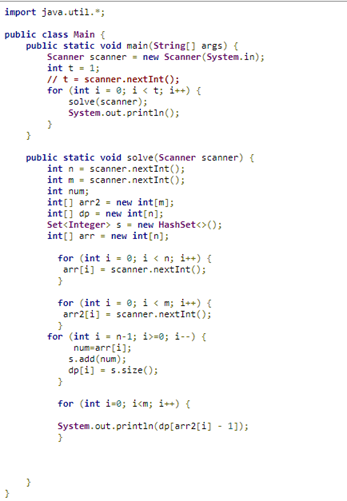
\includegraphics[width=0.5\linewidth]{Imagen1.png}
    \caption{
Hernández, G. D. A. (2023). \textit{Solución a B. Sereja and Suffixes Codeforces Problem 368B} [PNG]. Herramienta de Recortes.}
\end{figure}
Cabe destacar que también se uso programación dinámica para calcular todas las respuestas en una sola pasada de la colección, así el índice que se nos proporciona por la segunda colección será el índice que contenga la respuesta en nuestro arreglo de soluciones, en este caso se le resta uno para adecuarse a los índices de los arreglos que son de 0-n, porque los índices de la segunda colección son desde 1-n.
Como ya se dijo, la elección entre la clase \textit{HashSet, LinkedHashSet y TreeSet} para implementar la interfaz \textit{Set} en \textbf{Java} depende de nuestros requerimientos junto con el rendimiento y comportamiento que busquemos. Por ende, nos conviene tener en cuenta ciertos aspectos a la hora de elegir alguna de estas clases para nuestra aplicación.

\begin{itemize}
    \item \textbf{HashSet:}
    \begin{itemize}
    \item Se suele utilizar cuando se necesita una colección de elementos únicos sin tomar en cuenta el orden de inserción ni tampoco un orden específico para los elementos. Asimismo, es la clase más rápida para la mayoría de las operaciones, como inserción, eliminación y búsqueda.
    \item En lo que al rendimiento se refiere, un objeto de la clase \textit{HashSet} es altamente eficiente para las operaciones mencionadas anteriormente, ya que utiliza una tabla hash para el almacenamiento. Sin embargo, no garantiza ningún orden específico de los elementos.
    \end{itemize}
    \item LinkedHashSet:
    \begin{itemize}
    \item Se recomienda utilizar si quieres mantener el orden de inserción de los elementos, y en consecuencia los elementos también se pueden recuperar en el mismo orden en que se insertaron.
    \item En cuanto al rendimiento la clase\textit{ LinkedHashSet} es un poco más lenta que la clase\textit{ HashSet} debido a que mantiene el orden de inserción, pero es más rápida que la clase \textit{TreeSet}.
    \end{itemize}
    \item TreeSet:
    \begin{itemize}
    \item Se utiliza usualmente cuando necesitamos que los elementos se almacenen y recuperen de acuerdo con el orden natural o con algún orden personalizado. Por consiguiente, la clase T\textit{reeSet} garantiza que los elementos estén ordenados.
    \item Con relación al rendimiento de la clase \textit{TreeSet}, dado que esta utiliza un \textit{Red-Black Tree} para el almacenamiento, provoca que las operaciones de inserción, eliminación y búsqueda tengan un rendimiento ligeramente más lento que la clase \textit{HashSet} y \textit{LinkedHashSet.} No obstante, tener un orden nos puede ser muy útil para ciertas aplicaciones.
    \end{itemize}
\end{itemize}

\subsubsection{Interfaz Map}
Un Map es una estructura de datos que admite el par clave-valor para mapear los datos. Esta interfaz no admite claves duplicadas porque la misma clave no puede tener múltiples asignaciones; sin embargo, permite valores duplicados en claves diferentes. Un Map es útil cuando existen datos con los que queremos realizar operaciones en base a una clave. Además, la interfaz Map se puede implementar mediante diversas clases como HashMap, Hashtable y LinkedHashMap con la creación de una instancia de alguna de estas.
\paragraph{Clase HashMap}
Esta clase es una implementación de la interfaz Map basada en una tabla hash. Por ende, nos proporciona todas las operaciones opcionales de Map y permite valores null junto con claves null. Por otro lado, la clase HashMap es similar a la clase Hashtable, con la diferencia de que la clase HashMap no está sincronizada y permite valores nulos. Lamentablemente, esta clase no ofrece garantía en cuanto al orden del mapa; en particular, no garantiza que el orden se mantendrá constante en el tiempo.
Asimismo, esta implementación nos proporciona un rendimiento en tiempo constante para las operaciones básicas get y put, suponiendo que la función hash disperse los elementos adecuadamente entre los depósitos.
\paragraph{Clase Hashtable}
Esta clase implementa una tabla hash, que asigna claves a valores. Cualquier objeto no nulo se puede utilizar como clave o como valor. Para almacenar y recuperar objetos de una tabla hash con éxito, los objetos utilizados como claves deben implementar el método hashCode y el método equals.
Consecuentemente, una instancia de la clase Hashtable tiene dos parámetros que afectan su rendimiento: initial capacity y load factor. El load factor es la cantidad de depósitos en la tabla hash y la initial capacity es simplemente la capacidad en el momento en que se crea la tabla hash. Hay que tener en cuenta que la tabla hash está abierta: en el caso de una colisión, un único depósito almacena varias entradas, que deben buscarse secuencialmente. El load factor es una medida de qué tan llena se permite que esté la tabla hash antes de que su capacidad aumente automáticamente. Por lo anterior, los parámetros de initial capacity y load factor son meros consejos para la implementación.


\paragraph{Clase LinkedHashMap}
La clase implementa una tabla hash junto con una lista ligada de la interfaz Map, por lo cual, se cuenta con un orden de iteración predecible. Además, esta clase se diferencia de la clase HashMap porque mantiene una lista doblemente ligada que recorre todas sus entradas. Esta lista doblemente ligada define el orden de iteración, que normalmente es el orden en que se insertaron las claves en el mapa. Cabe destacar que el orden de inserción no se ve afectado si se vuelve a insertar una clave en el mapa.
Asimismo, la clase evita los pedidos no especificados y generalmente caóticos proporcionados por las clases HashMap y Hashtable, sin incurrir en el mayor costo asociado con TreeMap. Por consiguiente, esta clase se puede utilizar para producir una copia de un mapa que tenga el mismo orden que el original, sin importar la implementación del mapa original.
\subsubsection{Interfaz SortedMap}
La interfaz SortedMap amplía la interfaz Map con una estipulación adicional de un orden total de claves. Por ello, las claves se ordenan por orden natural o en base a un Comparator especificado en el momento de la construcción, de acuerdo con el constructor utilizado. En consecuencia, todas las claves deben ser comparables.
\paragraph{Clase Treemap}
Esta clase usa un\textit{ Red-Black Tree} basado en la interfaz \textit{NavigableMap} y \textit{SortedMap}, el cual se ordena en el orden natural de las Keys o por un comparador definido por el programador. Esta implementación garantiza un costo de tiempo de log(n) para las operaciones de búsqueda, obtención, inserción y eliminación de los elementos. Sin embargo, esta clase no está sincronizada. Por otra parte, dada su naturaleza al igual que el \textit{TreeSet} esta clase posee métodos exclusivos que nos permiten acceder a ciertos datos de manera más rápida.
\begin{itemize}
    \item \textbf{firstKey()} devuelve la clave del primer elemento en el mapa, que es la clave mínima en orden natural.
    \item \textbf{lastKey()} devuelve la clave del último elemento en el mapa, que es la clave máxima en orden natural.
    \item \textbf{headMap(K toKey)} devuelve una vista del mapa que contiene todas las entradas cuyas claves son menores que toKey.
    \item \textbf{tailMap(K fromKey)} devuelve una vista del mapa que contiene todas las entradas cuyas claves son mayores o iguales a fromKey.
    \item \textbf{subMap(K fromKey, K toKey)} devuelve una vista del mapa que contiene todas las entradas cuyas claves están en el rango [fromKey, toKey), es decir, desde fromKey (inclusivo) hasta toKey (exclusivo).
    \item \textbf{comparator()} devuelve el Comparator utilizado para ordenar las claves en el mapa. Si el mapa utiliza el orden natural, este método devolverá null.
\end{itemize}

\subsubsection{Aspectos a tomar en cuenta para elegir alguna de las clases de Map}
La elección entre las clases HashMap, Hashtable, LinkedHashMap o TreeMap para implementar la interfaz Map en Java depende de los requerimientos que se nos soliciten junto con el rendimiento y comportamiento que se busque. Por lo cual, nos conviene tener presentes ciertos aspectos al momento de elegir alguna de estas clases para nuestra aplicación.
\begin{itemize}
    \item HashMap:
    \begin{itemize}
    \item Se recomienda utilizar cuando necesites una estructura de datos de mapeo clave-valor con acceso rápido a los elementos. Es la elección predeterminada en la mayoría de los casos, ya que ofrece un buen equilibrio entre rendimiento y funcionalidad.
    \item El rendimiento de esta clase es altamente eficiente para la mayoría de las operaciones, como inserción, eliminación y búsqueda, pero no garantiza ningún orden específico de las claves.
    \end{itemize}
    \item Hashtable:
    \begin{itemize}
    \item Aunque la clase Hashtable es similar a la clase HashMap en términos de funcionalidad, se utiliza con menos frecuencia en aplicaciones modernas debido a su sincronización, que puede degradar el rendimiento en entornos multihilo. Por ello, si necesitas un mapa sincronizado, thread-safe, puedes optar por la clase Hashtable. De lo contrario, la clase HashMap es preferible.
    \item El rendimiento de la clase Hashtable es menor que el de la clase HashMap debido a la sincronización. Por ende, si no requieres de la sincronización, la clase HashMap será más rápida.
    \end{itemize}
    \item LinkedHashMap:
    \begin{itemize}
    \item Si deseas mantener el orden de inserción de las claves o el orden en el que se accede a los elementos, se recomienda utilizar la clase LinkedHashMap.
    \item El rendimiento de la clase LinkedHashMap es ligeramente más lento que el de la clase HashMap, ya que debe realizar un seguimiento del orden de inserción o acceso. Sin embargo, es más rápido que el de la clase TreeMap.
    \end{itemize}
    \item TreeMap:
    \begin{itemize}
    \item Se recomienda utilizar la clase TreeMap cuando requieras que las claves sean almacenadas de acuerdo al orden natural o de acuerdo con un orden personalizado. Por lo anterior, esta clase garantiza un orden ascendente o descendente de las claves.
    \item El rendimiento de la clase TreeMap es menos eficiente que el de las clases HashMap y LinkedHashMap en la mayoría de las operaciones debido a la estructura de árbol utilizada para mantener el orden. No obstante, ofrece la ventaja de un acceso ordenado a las claves.
    \end{itemize}
\end{itemize}
\chapter{Desarrollo}
\section*{EJERCICIOS DEL PROYECTO}
\subsection*{Búsqueda Lineal y Binaria en listas de objetos}
\begin{enumerate}
    \item Elaboración de Clases
    \begin{itemize}
        \item Elabora las clases necesarias donde definas los atributos y métodos de un objeto para crear el tipo de dato Alumno y el tipo de dato Asignatura. Asegúrate de considerar lo siguiente:
        \begin{itemize}
            \item Atributos privados.
            \item Acceso a los atributos a través de getters y setters.
            \item Constructor con parámetros.
        \end{itemize}
    \end{itemize}

    \item Clase Búsqueda Lineal
    \begin{itemize}
        \item Elabora una clase llamada BúsquedaLineal similar a la práctica 4, en la cual se implementarán métodos que devuelvan objetos y que reciban los siguientes parámetros:
        \begin{enumerate}
            \item Nombre (búsqueda por nombre del alumno).
            \item Clave (búsqueda por clave de la asignatura).
        \end{enumerate}
    \end{itemize}

    \item Clase Principal
    \begin{itemize}
        \item En la clase principal del proyecto, crea una lista de asignaturas y una lista de alumnos. Luego, comprueba el funcionamiento de los métodos realizados para las búsquedas.
    \end{itemize}

    \item Búsqueda Binaria (Opcional)
    \begin{itemize}
        \item Para obtener puntos extras en el proyecto, puedes realizar la búsqueda binaria. Deberás investigar cómo ordenar la lista de alumnos o la lista de asignaturas a partir de alguno de sus atributos y posteriormente aplicar el algoritmo de búsqueda binaria.
    \end{itemize}
\end{enumerate}
El algoritmo de búsqueda lineal en su esencia es sencillo, solo consta de recorrer toda la colección en busca de los elementos que coincidan con lo que buscamos, lo difícil fue la parte de implementación en el lenguaje Java pues se requirió de investigar y conocer cómo hacer distintas adaptación necesarias para la correcta ejecución del programa.
Para este ejercicio se crearon 2 paquetes, el paquete Escuela, el cual tiene las clases de Asignatura y Alumno lo que nos dará la posibilidad de crear los objetos necesarios para ser insertados en una lista y después buscarlos.
Y el paquete Búsquedas que poseen la búsqueda lineal y la búsqueda binaria.
\subsubsection{Descripción de clases}
\paragraph{Clase Alumno:}
Esta clase implementa el Comparable esto para definir que los objetos creados son comparables y asi admitir el método CompareTo.La clase posee 3 atributos un contador estático que determinara cuantos objetos Alumno hay, un String Alumno que contendrá el nombre del alumno y un entero en cuenta que poseerá el número de cuenta del alumno así diferenciando los objetos que posean el mismo nombre; dos constructores uno que inicializa todos los atributos y otro que solo inicializa el atributo nombre, este se utilizará posteriormente para la búsqueda binaria, posee métodos de acceso, un método de clase que sirve para llenar los datos del alumno, crea el objeto y lo devuelve para ser guardado en la lista; y 3 métodos sobreescritos, el ToString que contendrá los formatos de impresión del objeto, un método equals que comprobara que el atributo nombre sea igual al nombre que buscamos (esto para la búsqueda lineal), y un método compareTo que nos servirá para poder ordenar la lista y determinar si un objeto es mayor o menor que otro según qué atributo que nos servirá para crear la búsqueda binaria.


\paragraph{Clase Asignatura:}
Esta clase implementa el Comparable esto para definir que los objetos creados son comparables y así admitir el método CompareTo. La clase posee tres atributos un entero de clase contador que contendrá la cantidad de objetos creados, un String de instancia que contendrá el nombre de la asignatura y un entero de instancia que contendrá la clave de la asignatura; posee también sus métodos de acceso; dos constructores, uno para inicializar todos los atributos y otro para inicializar solo su clave (lo que nos servirá para la búsqueda binaria); un método de clase que sirve para instanciar el objeto, devolviéndolo ya con todos los datos solicitados; 3 métodos sobrescritos, el método ToString que maneja el formato de impresión del objeto y sus atributos, el método equals que servirá para en la búsqueda lineal solo comparar las claves y determinar si el objeto comparte la misma clave o no, y el método CompareTo que nos servirá para poder determinar cuando un objeto es mayor que otro según el atributo elegido para comparar esto nos servirá para la búsqueda binaria.
\paragraph{Clase Main:}
Esta clase es el menú donde se ejecutarán todas las opciones, este menú contiene dos Linked List una de alumnos y otra de asignaturas para tener guardados todos los objetos en los que se buscará, posteriormente se despliega un menú que muestra todas las opciones disponibles:

\begin{figure}[htbp]
\centering
\begin{lstlisting}[language=Java, frame=lines, framesep=2mm, basicstyle=\footnotesize\ttfamily, numbers=left]
      do{
                Utilerias.clearScreen();
                System.out.println("Bienvenido al sistema de busqueda de alumnos");
                System.out.println("Escoge una opcion");
                System.out.println("1.-Agregar Alumno");
                System.out.println("2.-Agregar materia");
                System.out.println("3.-Imprimir Listas");
                System.out.println("4.-Busqueda lineal");
                System.out.println("5.-Busqueda Binaria");
                s=cin.nextInt();
                switch (s) {
                case 1: a.add(Alumno.crear());break;
                case 2: m.add(Asignatura.crear()); break;
                case 3: System.out.println("1.-Lista Alumnos 2.-Lista Materias"); s=cin.nextInt(); if(s==1){Imprimir(a);}else{Imprimir(m);} ; break;
                case 4: BL.menu(a, m);break;
                case 5: BB.menu(a, m);break;
                default:
                return;
            }
        }while(true);
\end{lstlisting}
\caption{Menú de opciones}
\end{figure}
\subsubsection{Búsqueda Lineal}
Para la búsqueda lineal, en su clase se crearon los atributos privados:\\
\begin{figure}[htbp]
\centering
\begin{lstlisting}[language=Java, frame=lines, framesep=2mm, basicstyle=\footnotesize\ttfamily, numbers=left]
     private boolean rb;
     private LinkedList<Integer> ind;
     private int c=0;
\end{lstlisting}
\caption{Atributos clase búsqueda lineal}
\end{figure}

Estos atributos nos servirán para guardar los datos que necesitamos, es decir, si el objeto es encontrado en rb se guardará un True, en la LinkedList se guardaran todas las posiciones en las que el objeto es encontrado y en el entero se guardaran la cantidad de veces que el elemento haya sido encontrado.
\newpage
El método que realiza la búsqueda llamado BLB, devuelve un objeto de tipo BL, esto porque el objeto BL será aquel que contenga los atributos mencionados y los mostrará como salida en el programa.

El método BLB, recibe un Object y una List<?>, es decir, recibe dos tipos genéricos uno de objeto y otro de lista, su propósito es que este mismo método pueda recibir una lista de Asignaturas o una lista de Alumnos y el objeto genérico recibe como objeto el atributo que se va a comparar para hacer la búsqueda, en caso de un Alumno recibirá un String y en caso de Asignatura recibirá un Integer.
La parte esencial del código es la siguiente:             
\begin{figure}[htbp]
\centering
\begin{lstlisting}[language=Java, frame=lines, framesep=2mm, basicstyle=\footnotesize\ttfamily, numbers=left]
for (Object i : list) {
    if (i.equals(v)) {
        b = true;
        count++;
        index.add(j);
    }
    j++;
}
BL OBL = new BL(b, index, count);
return OBL;
\end{lstlisting}
\caption{Algoritmo de búsqueda Lineal}
\end{figure}
\\Esta parte del código llena los atributos que posteriormente construirán el objeto mencionado para finalmente devolverlo:
Algo a destacar es el método equals, pues este método es que nos sirve para comparar el atributo con lo que estemos buscando para usarlo fue necesario sobrescribir este método tanto en la clase de Asignatura como en la Clase Alumno quedando de la siguiente manera.
\begin{figure}[htbp]
\centering
\begin{lstlisting}[language=Java, frame=lines, framesep=2mm, basicstyle=\footnotesize\ttfamily, numbers=left]
    @Override
    public boolean equals(Object obj) {
    return this.getAlumno().equals((String)obj);
    }
\end{lstlisting}
\caption{Método sobrescrito de Alumno: equals}
\end{figure}
\\Como se ve, recibe un objeto genérico, para este caso se sabe que lo que compararemos será el nombre del alumno, es decir, un String por lo que el objeto genérico se castea para convertirse a un objeto de tipo String, una vez esto se utiliza el método equals de la clase String para determinar si ambos Strings son iguales; el método sobrescrito solo hace que lo que se evalúe sea el atributo nombre del objeto, para esto el getter getAlumno devuelve el nombre del alumno el cual es una String, este String tiene su propio método equals para determinar si dos Strings son iguales por lo que se usa con el objeto genérico casteado/convertido a una String si son iguales el método devolverá un true y si no un false.
Esta misma lógica se aplica para el equals de Asignatura únicamente que aquí casteamos el objeto a un Integer y lo pasamos a entero para que pueda ser comparado de la manera usual:
\begin{figure}[htbp]
\centering
\begin{lstlisting}[language=Java, frame=lines, framesep=2mm, basicstyle=\footnotesize\ttfamily, numbers=left]
    @Override
    public boolean equals(Object obj) {
        Integer entero = (Integer) obj;      
    return this.clave == entero.intValue(); 
}
\end{lstlisting}
\caption{Método sobrescrito de Asignatura: equals}
\end{figure}
Una vez esto en la clase de la búsqueda lineal se tiene un método de clase llamado menú, el cual recibirá las dos listas, tanto la de alumnos como la de asignaturas y se crearán los dos genéricos (lista y objeto), una vez esto se le solicita al alumno que escoja que quiere buscar si escoge alumno la lista genérica tomará a la lista de alumnos y el objeto genérico recibe un String, si escoge Asignatura la lista genérica tomara la lista de asignaturas y el objeto recibirá un Integer.
Después de esto se ejecuta el método BLB explicado anteriormente y el objeto devuelto será guardado en un objeto de tipo BL(búsqueda lineal) llamado OBL(Objeto Búsqueda Lineal).

Ahora el usuario tendrá la posibilidad de escoger que quiere mostrar
\begin{enumerate}
    \item Búsqueda Booleana (Encontrado, No encontrado)
    \item Índice encontrado (Los índices de la lista en donde se localiza el objeto)
    \item Cuántas veces fue encontrado (Mostrará la cantidad de incidencias que tenga el objeto)
    \item Imprime todos los datos.(Mostrara el numero de veces, los índices y los objetos en cada índice pues estos pueden tener sus demás atributos diferentes)
\end{enumerate}
\paragraph{Método sistema de impresión:}
Este método es interesante pues es un método de instancia, el cual recibirá la lista original y utilizara los atributos llenados en el objeto para ir imprimiendo todos los índices de los objetos encontrados, recibe una lista genérica por lo que puede usarse para imprimir cualquier objeto tanto Alumno como Asignatura y emplea el método ToString para imprimir todos los atributos del objeto localizado.
\newpage
\subsubsection{Búsqueda Binaria:}
Para la búsqueda binaria no se empleó ningún atributo de instancia o clase, pues todas las respuestas son generadas por los métodos de clase creados, solo tiene un atributo de clase que es el scanner que se usará para el registro de datos.
\paragraph{Métodos CompereTo():}
Estos métodos son esenciales para que la ejecución del algoritmo de búsqueda binaria funcione, pues es lo que determina cuando un objeto es mayor o menor que otro caso, para esto se implementó la interfaz Comparable que habilita el método CompareTo para sobrescribirlo según lo que queramos evaluar.
Para la clase Alumno quedó sobrescrito de tal manera que solo evalúa el atributo que contiene el nombre del alumno:
\begin{figure}[htbp]
\centering
\begin{lstlisting}[language=Java, frame=lines, framesep=2mm, basicstyle=\footnotesize\ttfamily, numbers=left]
    @Override
    public int compareTo(Alumno A2) {
       return this.getAlumno().compareTo(A2.getAlumno());
    }
\end{lstlisting}
\caption{Método sobrescrito de Alumno: CompareTo}
\end{figure}
Se usa el getter para obtener el String y usar el propio compareTo del string con el string del otro objeto a recibir, así retornado el resultado que puede ser positivo para mayor que, negativo para menor que y cero para valores iguales.
Para la clase Asignatura quedo sobrescrito de tal manera que solo use la clave para compararlo:
\begin{figure}[htbp]
\centering
\begin{lstlisting}[language=Java, frame=lines, framesep=2mm, basicstyle=\footnotesize\ttfamily, numbers=left]
    @Override
    public int compareTo(Asignatura A2) {
        return Integer.compare(this.getClave(), A2.getClave());
    }
\end{lstlisting}
\caption{Método sobrescrito de Asignatura: CompareTo}
\end{figure}
\\Utilizando el compare de la clase Integer para comparar los dos enteros, devolviendo así un valor negativo para menor que, un valor positivo para mayor que y cero para valores iguales. 
\newpage 
\paragraph{Método BBI (Búsqueda Binaria index)}
Este método devolverá un entero y usa \(<\)T extends Comparable \(<\)T\(>\)\(>\) para definir un objeto genérico comparable, pues recibirá dos parámetros de ese tipo un objeto genérico comparable v y una lista de objetos comparables list, esta lista cabe destacar que debe estar ordenada, para esto se definió a todas las clases como comparables (lo anteriormente mencionado) y se reescribieron los métodos de CompareTo, en el caso de Asignatura se reescribir de tal manera que solo compara las claves de ambos objetos, y para el caso de Alumno solo compare el nombre de cada alumno, así al usar Collections.Sort() este método se basará en los métodos CompareTo sobrescritos para ir ordenando las colecciones.
El método inicializa una variable b en -1 pues esta es la variable que registra el índice por lo que si no lo encuentra devolverá un -1 que indicará que no hay tal objeto buscado, si la lista está vacía retorna -1.
Después define una variable mid el cual es el valor que se encuentra en medio de la lista y empieza el algoritmo, se obtiene el objeto en el index mid y a este se le hace un CompareTo con el objeto genérico que fue recibido de la siguiente manera:
\begin{figure}[htbp]
\centering
\begin{lstlisting}[language=Java, frame=lines, framesep=2mm, basicstyle=\footnotesize\ttfamily, numbers=left]
 if(v.compareTo(list.get(mid))==0){
                b=mid;
              return b;      
        }else if(v.compareTo(list.get(mid))>0){
            aux+=BBI(v, list.subList(mid+1, list.size()));
            if(aux==-1){
                 return -1;  
            }else{
              
                b=mid+1+aux;
            }
        }else if(v.compareTo(list.get(mid))<0){
            b=0;
            b+=BBI(v, list.subList(0,mid));
        }
\end{lstlisting}
\caption{Método sobrescrito de Asignatura: CompareTo}
\end{figure}
Este método lo que hace es regresar un valor negativo si el objeto es menor, un valor positivo si es mayor y cero si los valores son iguales, por lo que así define cómo se va partiendo la lista en cada llamada recursiva.

Para cada llamada recursiva se va definiendo nuevamente b para ir alineando el index que debe llevar según como se parta la lista en caso de que la lista vaya hacia los indices después del valor central se usa una variable auxiliar que evalúa si el valor si fue encontrado para que la variable que registra el índice se ajuste y si no devuelva -1 sin el ajuste del índice pues no es necesario ya que no encontró el valor.

Al final devuelve el index en el que encontró el elemento, este elemento puede ser el de en medio, la primera incidencia o la última incidencia por lo que para encontrarlas todas se usa el método EncontrarIndicesdetodaslasincidencias.
\paragraph{Metodo Encontrar Índices de todas las incidencias:}
Este método devuelve una lista de enteros, recibe un objeto genérico comparable, una lista de objetos genéricos comparables y el índice generado por el metodo de busqueda binaria; solo funciona si se encontró por lo menos una incidencia en el método de búsqueda binaria, es decir, si el valor regresado por el método de búsqueda binaria es mayor o igual que cero.
Sino devolverá la lista vacía.
Se crea una Linkedlist llamada index.
Añade el índice recibido como parámetro a index y define dos enteros lb (límite izquierdo) y rbound (límite derecho) los cuales se mueven desde donde está el indice encontrado, hacia la izquierda en caso de lb y hasta la derecha en caso de rb así hasta que los índices se topen con un valor distinto al que se busca para esto se utilizan los métodos compareto ya mencionados anteriormente, cada que encuentra un elemento igual añade la variable de límite a la lista index pues estas variables representan los índices de la lista, así hasta que ambos límites se hayan encontrado con un valor distinto al buscado o se hayan llegado a los límites de la lista.
Retorna la lista index la cual contiene todos los índices localizados.
\paragraph{Menú:}
El método recibe dos listas, la lista de alumnos y la lista de asignaturas, define un objeto genérico v una linkedlist de objetos genéricos comparables, sortea ambas listas con ayuda del collections.sort().
Le solicita al usuario que decidirá buscar, en caso de que busque un alumno por nombre la lista de alumnos se casteara a (LinkedList\(<\)T\(>\)) y se asignará a la lista genérica, aquí es donde entra el constructor de que solo inicializa el nombre pues, se necesitará que este objeto genérico contenga un objeto del mismo tipo que se va a buscar, pues el método compareto solo admite comparaciones con objetos del mismo tipo, pero solo inicializamos el nombre porque es el único atributo que consideraremos, en caso de que el usuario escoja buscar asignatura por nombre realiza lo mismo pero con el constructor de asignatura.
Una vez esto, imprime la lista ordenada y ejecuta el método de ordenamiento por búsqueda binaria, devolviendo el primer índice encontrado, posteriormente se crea una lista de enteros denominada Index que será la lista que devolverá el método que encontrará las demás incidencias.
Ahora el usuario tendrá la posibilidad de escoger que quiere mostrar
\begin{enumerate}
    \item Búsqueda Booleana (Encontrado, No encontrado)
    \item Índice encontrado (Los índices y los objetos en cada índice pues estos pueden tener sus demás atributos diferentes)
    \item Cuántas veces fue encontrado (Mostrara el numero de veces que fue encontrado)
    \item Imprime todos los datos.(Mostrara el numero de veces, los índices y los objetos en cada índice pues estos pueden tener sus demás atributos diferentes)
\end{enumerate}
\paragraph{Método sistema de impresión:}
Este método recibe la lista de índices y una lista de genéricos para así imprimir todos los índices que contienen tal objeto y el objeto que se encuentra en ese índice utilizando el método toString.
\subsubsection{Ejecución:}

\begin{figure}[h]
    \centering
    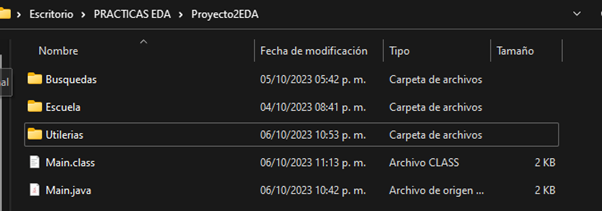
\includegraphics[width=1\linewidth]{Imagen3.png}
    \caption{Paquetes y Clase Main:}
  
\end{figure}
\begin{figure}[h]
    \centering
    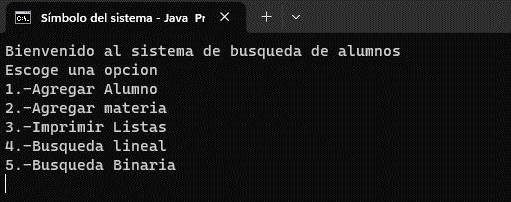
\includegraphics[width=1\linewidth]{Imagen4.png}
    \caption{Menú}
\end{figure}
\begin{figure}[h]
    \centering
    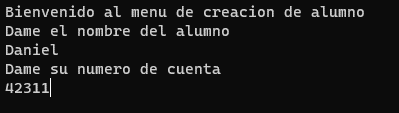
\includegraphics[width=1\linewidth]{Imagen5.png}
    \caption{Creación de Alumno Daniel}

\end{figure}
\begin{figure}[h]
    \centering
    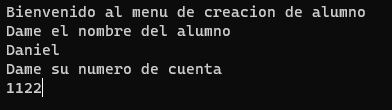
\includegraphics[width=1\linewidth]{Imagen6.png}
    \caption{Creación Alumno Daniel 2}
\end{figure}
\begin{figure}[h]
    \centering
    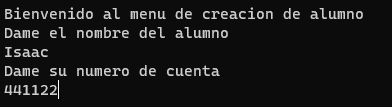
\includegraphics[width=1\linewidth]{Imagen7.png}
    \caption{Creacion Alumno Isaac}
    
\end{figure}
\begin{figure}[h]
    \centering
    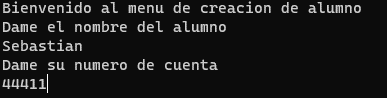
\includegraphics[width=1\linewidth]{Imagen8.png}
    \caption{Creación Alumno Sebastian}
    
\end{figure}
\begin{figure}[h]
    \centering
    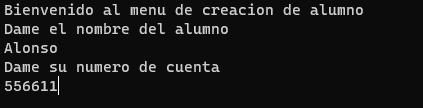
\includegraphics[width=1\linewidth]{Imagen9.png}
    \caption{Creación Alumno Alonso}
    
\end{figure}
\begin{figure}[h]
    \centering
    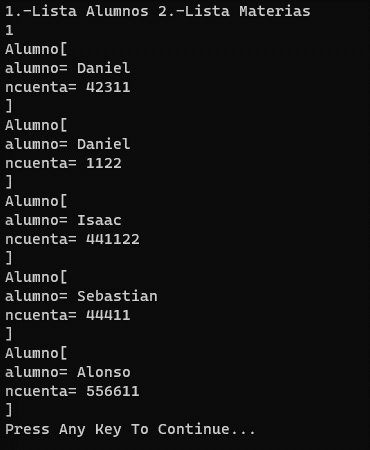
\includegraphics[width=1\linewidth]{Imagen10.png}
    \caption{Impresion}
    
\end{figure}

\begin{figure}[h]
    \centering
    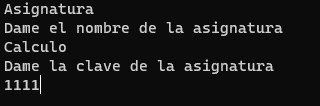
\includegraphics[width=1\linewidth]{Imagen11.png}
    \caption{Creacion asignatura Calculo}
    
\end{figure}
\begin{figure}
    \centering
    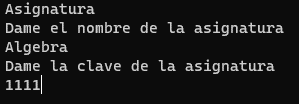
\includegraphics[width=1\linewidth]{Imagen12.png}
    \caption{Creación Asignatura Álgebra}
    
\end{figure}
\begin{figure}
    \centering
    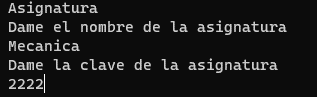
\includegraphics[width=1\linewidth]{Imagen13.png}
    \caption{Creación materia Mecánica}
    
\end{figure}[h]
\begin{figure}
    \centering
    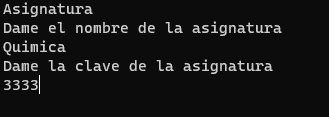
\includegraphics[width=1\linewidth]{Imagen14.png}
    \caption{Creación materia Química}
    
\end{figure}
\begin{figure}
    \centering
    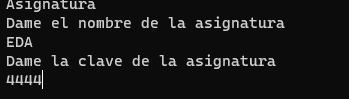
\includegraphics[width=1\linewidth]{Imagen15.png}
    \caption{Creación materia EDA}
    
\end{figure}
\begin{figure}
    \centering
    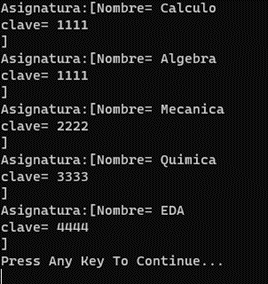
\includegraphics[width=1\linewidth]{Imagen16.png}
    \caption{Impresión de las Asignaturas }
    
\end{figure}
\begin{figure}
    \centering
    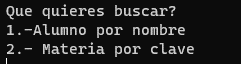
\includegraphics[width=1\linewidth]{Imagen17.png}
    \caption{Menú Búsqueda Lineal}
    
\end{figure}
\begin{figure}
    \centering
    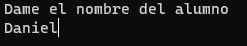
\includegraphics[width=1\linewidth]{Imagen18.png}
    \caption{Solicitud de Búsqueda por nombre a Daniel}
    
\end{figure}
\begin{figure}
    \centering
    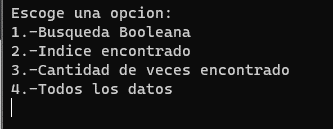
\includegraphics[width=1\linewidth]{Imagen19.png}
    \caption{Menú 2 Búsqueda Lineal}
    
\end{figure}
\begin{figure}
    \centering
    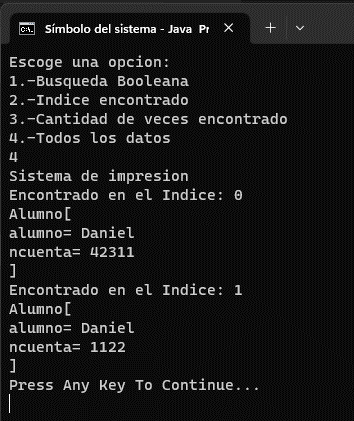
\includegraphics[width=1\linewidth]{Imagen20.png}
    \caption{Impresión de todos los datos}
    
\end{figure}

\begin{figure}
    \centering
    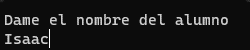
\includegraphics[width=1\linewidth]{Imagen21.png}
    \caption{Solicitud de búsqueda por nombre de Isaac}
    
\end{figure}
\begin{figure}
    \centering
    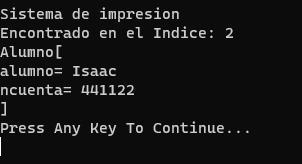
\includegraphics[width=1\linewidth]{Imagen22.png}
    \caption{Impresión de todos los datos}
    
\end{figure}
\begin{figure}
    \centering
    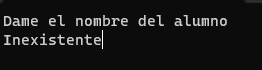
\includegraphics[width=1\linewidth]{Imagen23.png}
    \caption{Búsqueda Lineal por nombre de alumno inexistente }
\end{figure}
\begin{figure}
    \centering
    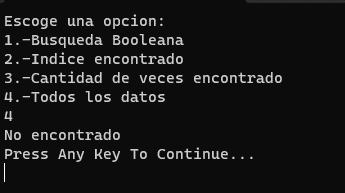
\includegraphics[width=1\linewidth]{Imagen24.png}
    \caption{Impresión de todos los datos}
\end{figure}

\begin{figure}
    \centering
    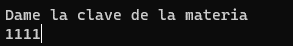
\includegraphics[width=1\linewidth]{Imagen25.png}
    \caption{Búsqueda de materia con Clave 1111}
    
\end{figure}
\begin{figure}
    \centering
    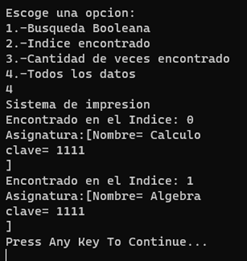
\includegraphics[width=1\linewidth]{Imagen26.png}
    \caption{Impresión de todos los datos}
\end{figure}
\begin{figure}
    \centering
    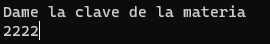
\includegraphics[width=1\linewidth]{Imagen27.png}
    \caption{Búsqueda de materia con Clave 2222}
    
\end{figure}
\begin{figure}
    \centering
    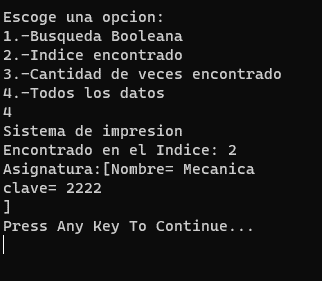
\includegraphics[width=1\linewidth]{Imagen28.png}
    \caption{Impresión de todos los datos}
    
\end{figure}
\begin{figure}
    \centering
    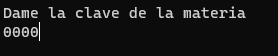
\includegraphics[width=1\linewidth]{Imagen29.png}
    \caption{Búsqueda de una clave inexistente}
    
\end{figure}
\begin{figure}
    \centering
    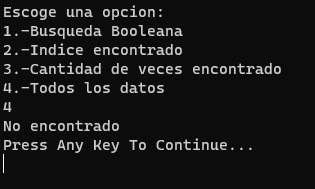
\includegraphics[width=1\linewidth]{Imagen30.png}
    \caption{Impresión de todos los datos}
    
\end{figure}




\chapter{Conclusiones}
\textbf{Hernandez Gallardo Daniel Alonso} \\
\newpage
\textbf{Perez Osorio Luis Eduardo} \\

\newpage
\textbf{Valle Chavez Anton Yael} \\
\newpage
\nocite{*}
  \newpage
\bibliography{citas.bib}

\end{document}
